\section{Energy resolution boost}
\label{Result}
Assume the PE counts $N$ on a PMT with PDE $\eta$ for an event with visible energy $E$ obeys Poisson distribution $\pi(\lambda_N=K\eta E)$, in which $K$ is a factor related to light yield and light transportation. The output total charge $\sum{Q}$ is a compound Poisson random variable with the expectation $\mathrm{E}[\sum{Q}]=\lambda_N\mathrm{E}[Q]$ and variance $\mathrm{Var}[\sum{Q}]=\mathrm{E}^2[Q]\lambda_N+\lambda_N\mathrm{Var}[Q]$.

The energy $E$ is estimated as $\hat{E}=\frac{\sum{Q}}{K\eta\mathrm{E}[Q]}$ with its resolution being

\begin{equation}
    \frac{\sqrt{\mathrm{Var}[\hat{E}]}}{\mathrm{E}[\hat{E}]}=\frac{\sqrt{\mathrm{E}^2[Q]\lambda_N+\lambda_N\mathrm{Var}[Q]}}{\lambda_N\mathrm{E}[Q]}=\frac{\sqrt{1+\frac{\mathrm{Var}[Q]}{\mathrm{E}^2[Q]}}}{\sqrt{K\eta E}}.
\end{equation}

The PMT specific factors are $\eta$ (proportional to relative PDE $\eta^0$) and $\frac{\mathrm{Var}[Q]}{\mathrm{E}^2[Q]}$ (estimated by sample resolutions $\nu^2$ in sec.~\ref{sec:noisegain}). The \emph{figure of merit} $M_{E}\equiv\sqrt{({1+\nu^2})/{\eta^0}}$ of the reference and 9 MCP PMTs are as shown in Fig.~\ref{fig:EnergyResolution}. Despite the long tail in the charge distribution, the boost of PDE of MCP-PMTs leads to a 10\% better $M_{E}$. We are developing an advanced waveform analysis method to model the charge distribution and count PEs that may eliminate the long-tail degradation on energy resolution.
\begin{figure}[!htbp]
    \centering
    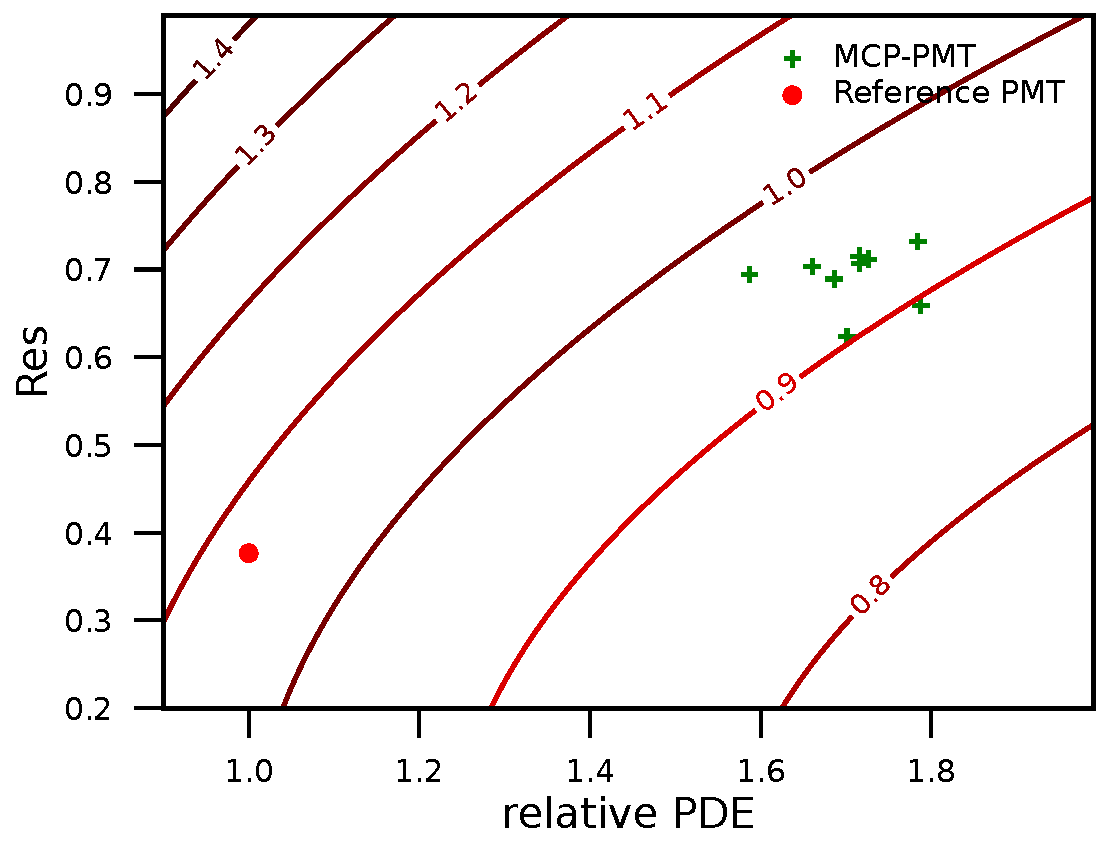
\includegraphics[width=\MF\textwidth]{figures/result/resolution.pdf}
    \caption{Contour map of $\nu_{E}$ as a function of the \emph{sample resolution} $\nu$ and the relative PDE. The relative PDE of reference PMT is 1.}
    \label{fig:EnergyResolution}
\end{figure}
